
\subsubsection{Cadre Général}


À chaque fois que le module reçoit un environnement annoté, celui-ci effectue une mise à jour des probabilités d'apparition d'une annotation en fonction d'une forme.
\[ P(Annotation|Forme) = \frac{P(Forme|Annotation) \times P(Annotation)}{P(Forme)} \]

Par exemple, imaginons que nous souhaitons entraîner notre IA à identifier des formes géométrique basique : rond, carré, croix et triangle. Admettons que notre IA est capable de reconnaître dans son environnement les formes correspondantes mais qu'elle ne sait pas les associer aux annotations correspondantes. Nous pouvons représenter cette état par le tableau représenté en figure \ref{img_annotations}.

\begin{figure}[H] 
  \begin{center}
    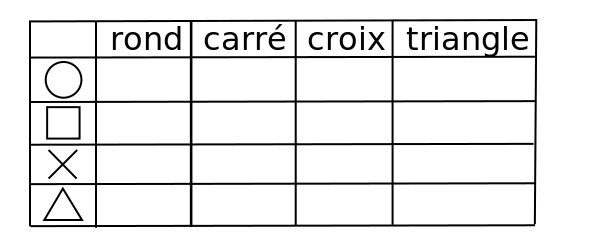
\includegraphics[width=0.5\textwidth]{files/raisonneur/annotations} 
  \end{center}
\caption{Association forme-annotations} 
\label{img_annotations}
\end{figure}

À partir de là, notre IA doit apprendre de ces expériences et pour ce faire elle doit mettre à jour les probabilités qu'une annotation soit rattachée à un environnement à chaque environnement rencontré. Par exemple, sur la figure \ref{img_annotations_1} nous pouvons voir qu'un environnement présentant la forme \og{} rond \fg{} et correctement annoté mettra à jour les probabilités de cette forme comme illustré.

\begin{figure}[H] 
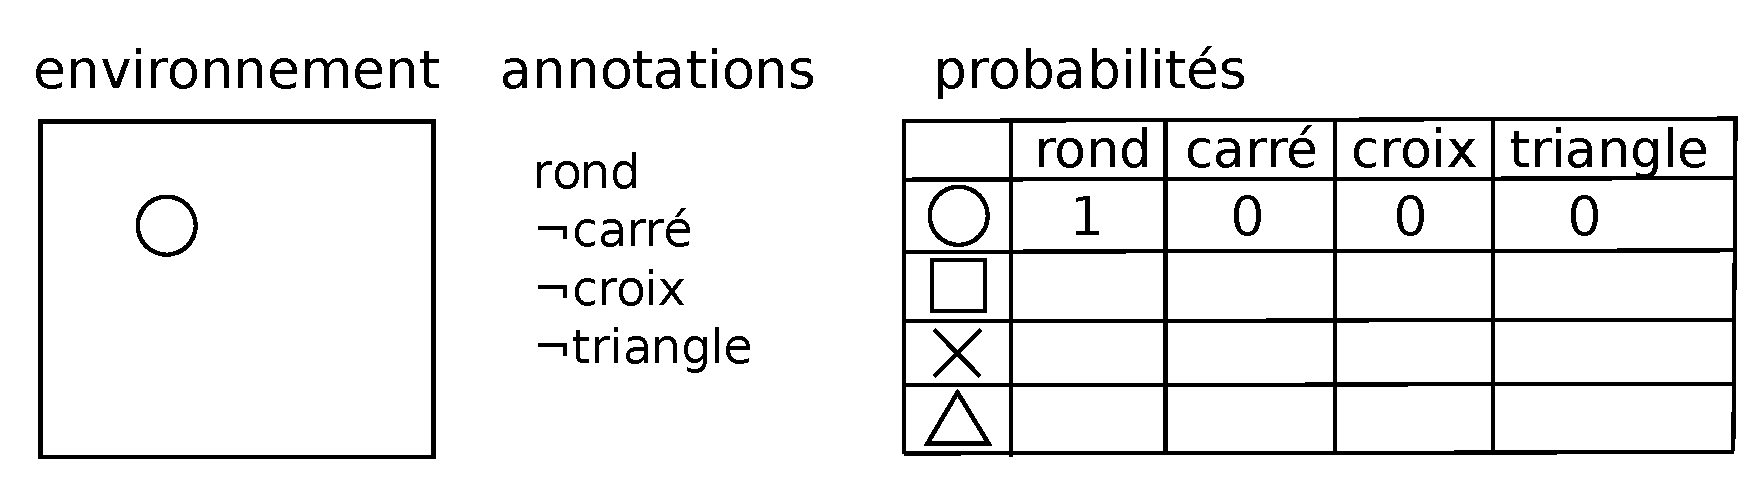
\includegraphics[width=\textwidth]{files/raisonneur/annotations_1} 
\caption{Association forme-concept 1} 
\label{img_annotations_1}
\end{figure}

De même pour un environnement présentant un ensemble de forme, comme sur la figure \ref{img_annotations_2}. Il existe alors une ambiguïté car le système ne peut savoir quelle forme est responsable de quelle annotation.  

\begin{figure}[H] 
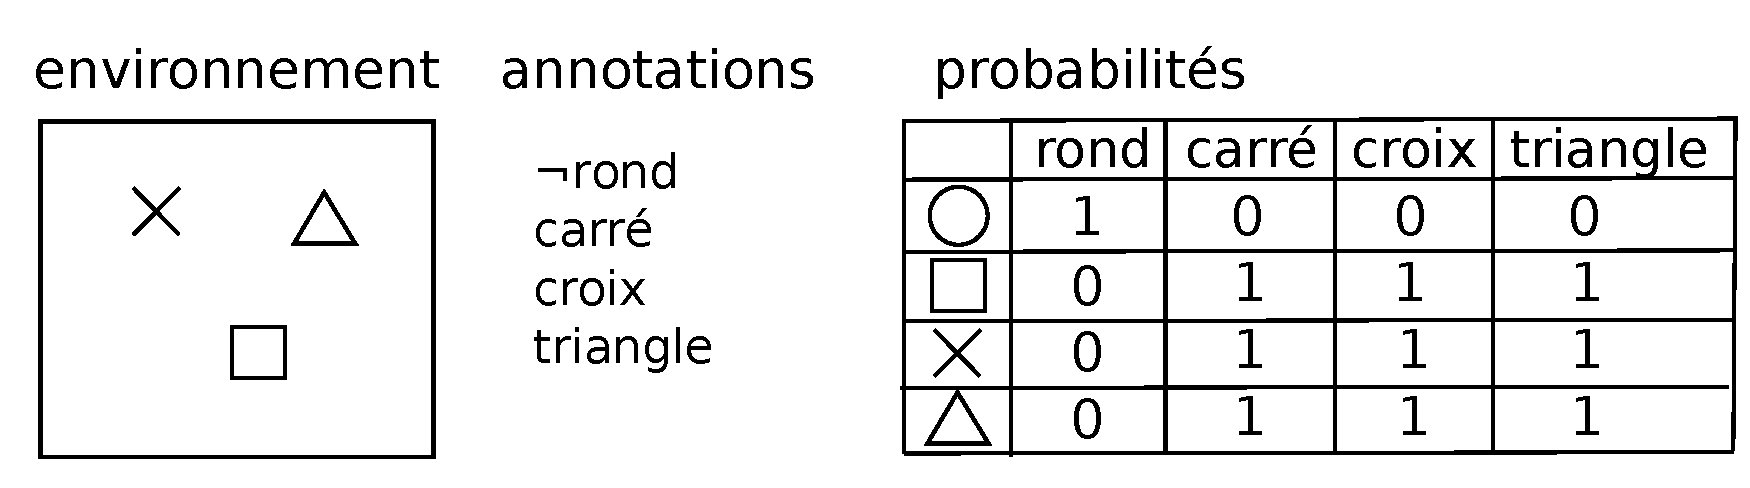
\includegraphics[width=\textwidth]{files/raisonneur/annotations_2} 
\caption{Association forme-concept 2} 
\label{img_annotations_2}
\end{figure}

Cependant, cette ambiguïté sera lever par l'expérience qui confrontera le système avec des ensembles variés de formes. En conséquence, seul l'annotation correct pour chaque forme gardera une probabilité certaine comme nous pouvons l'observer sur les figures \ref{img_annotations_3}, \ref{img_annotations_4} et \ref{img_annotations_5} qui illustrent l'évolution du système. 

\begin{figure}[H] 
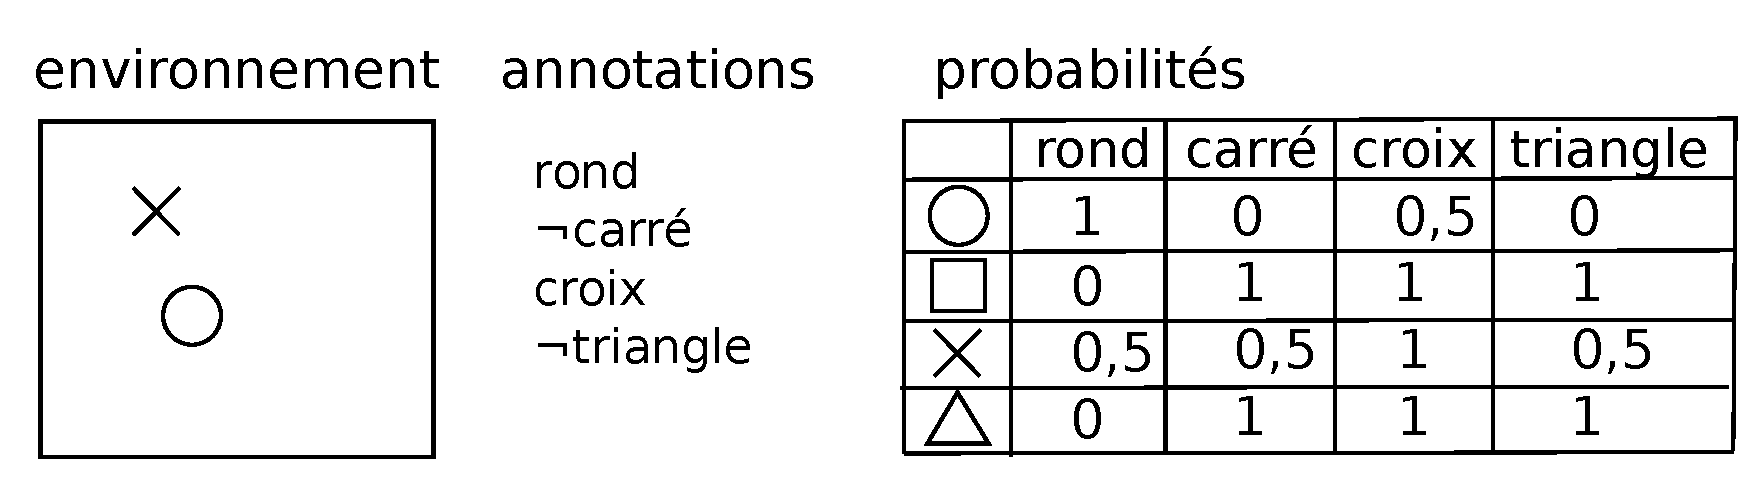
\includegraphics[width=\textwidth]{files/raisonneur/annotations_3} 
\caption{Association forme-concept 3} 
\label{img_annotations_3}
\end{figure}

\begin{figure}[H] 
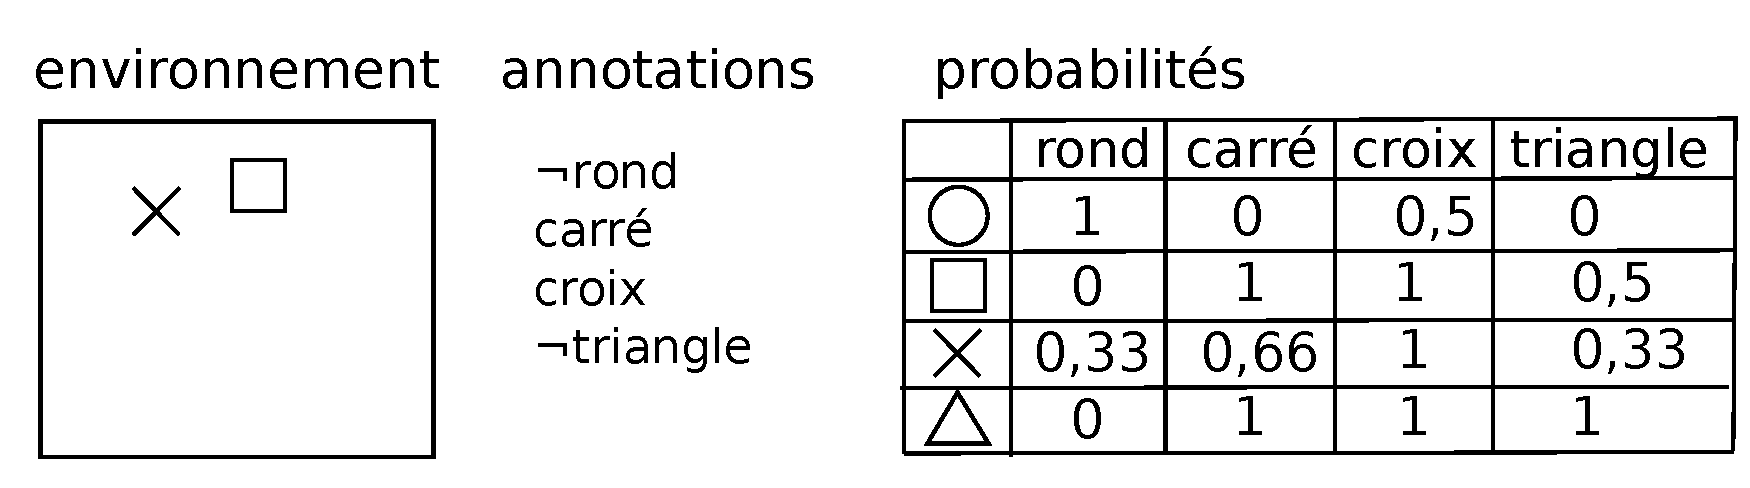
\includegraphics[width=\textwidth]{files/raisonneur/annotations_4} 
\caption{Association forme-concept 4} 
\label{img_annotations_4}
\end{figure}

\begin{figure}[H] 
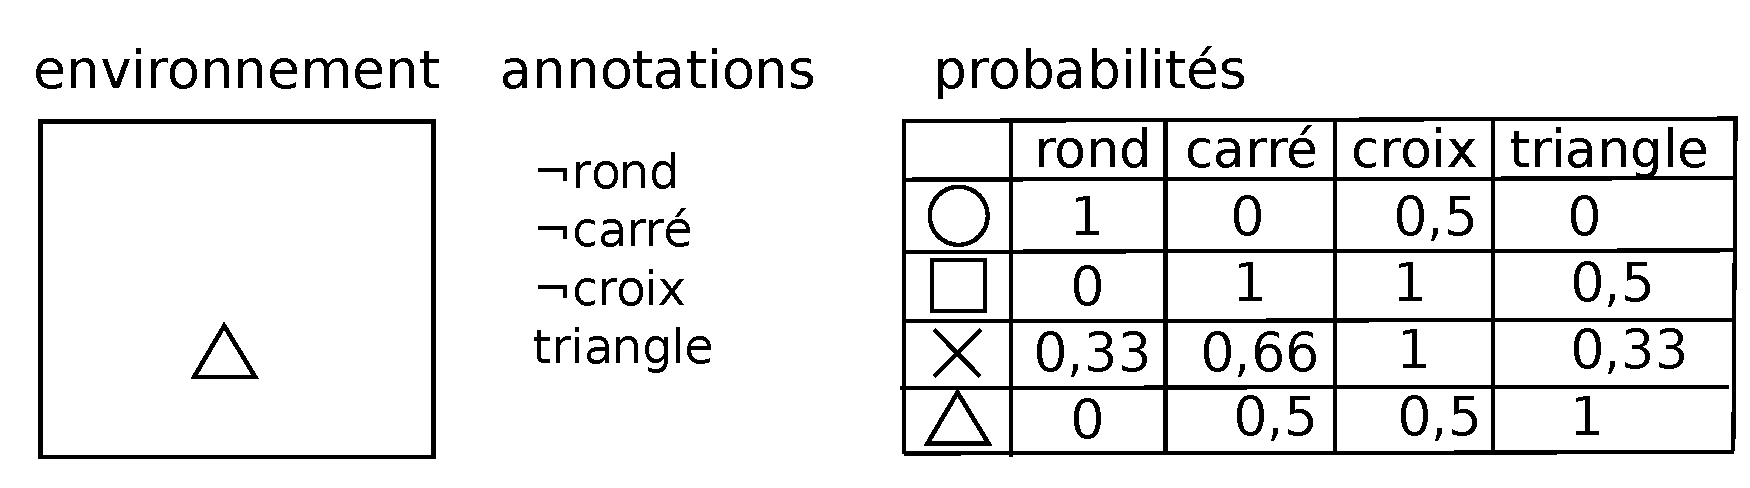
\includegraphics[width=\textwidth]{files/raisonneur/annotations_5} 
\caption{Association forme-concept 5} 
\label{img_annotations_5}
\end{figure}

Il est important de noter que la certitude, représenté par une probabilité de un, ne peut être garanti que si les annotations fournit au système lors de sa période d'apprentissage sont sans erreur. Cependant, une erreur d'annotations lors de l'apprentissage, certes diminuerai la probabilité associé à l'annotation correct mais, pour vu que le jeux d'apprentissage soit assez grands, celle-ci resterai la plus probable.

\subsubsection{Application aux jeux de plateau}

Dans le cadre des jeux de plateau deux annotations seront fourni \og victoire \fg{} et \og défaite \fg{}, et bien évidement \og victoire$\rightarrow{}\neg{}$défaite \fg{} et \og défaite$\rightarrow{}\neg{}$victoire \fg{}. Ces annotations doivent être fournies directement par l'environnement sans intervention humaine, nous sommes donc sur de l'apprentissage par renforcement.
